\documentclass[a4paper]{article}
\usepackage[utf8]{inputenc}
\usepackage{lmodern}
\usepackage[T1]{fontenc}
%\usepackage[italian]{babel}
\usepackage{microtype}
\usepackage{acronym}
\usepackage{mathtools}
\usepackage{amsfonts}
\usepackage{amssymb}
\usepackage{amsthm}
\usepackage[hidelinks,breaklinks=true]{hyperref}
\usepackage{xcolor}
\usepackage{listings}
\usepackage{algorithm}
\usepackage[noend]{algpseudocode}

\newcommand{\me}{\ensuremath{\mathrm{e}}}
\newcommand{\md}{\ensuremath{\mathrm{d}}}
\newcommand{\tc}{\ensuremath{\mathrm{t.c.:}\quad}}
\newcommand{\expected}[1]{\ensuremath{\mathrm{\textbf{E}}\left[#1\right]}}
\newcommand{\variance}[1]{\ensuremath{\mathrm{\textbf{Var}}\left(#1\right)}}
\newcommand{\prob}[1]{\ensuremath{\mathrm{\textbf{P}}\left(#1\right)}}
%\newcommand{\max}[1]{\ensuremath{\mathrm{max}\left(#1\right)}}
\newcommand{\abs}[1]{\ensuremath{\left|#1\right|}}
\newcommand{\mR}{\ensuremath{\mathbb{R}}}
\newcommand{\codei}[1]{\texttt{#1}}

%\newtheorem{defi}{Definizione}[chapter]

\lstset{inputpath=src}
\lstdefinestyle{customPy}{
 language=python,
 showstringspaces=false,
 basicstyle=\footnotesize\ttfamily,
 keywordstyle=\bfseries\color{green!40!black},
 commentstyle=\itshape\color{purple!40!black},
 identifierstyle=\color{blue},
 stringstyle=\color{orange},
}

%\DeclarePairedDelimiter\abs{\lvert}{\rvert}

\author{
  {\Large Stefano Martina}\\
  {\small stefano.martina@stud.unifi.it}\\
  Universit\`a degli Studi di Firenze\\
  Scuola di Scienze Matematiche, Fisiche e Naturali\\
  Corso magistrale di Informatica
}
\title{{\Huge\bfseries A simulated annealing approach to solve path
    planning}}%\\{\large\bfseries Esame di Laboratorio di Fisica Computazionale}}

\begin{document}
\maketitle
\thispagestyle{empty}
\vfill
\begin{abstract}
  This work is about a simulated annealing method for performing path
  planning.
\end{abstract}

\section{Introduction}
The \emph{Path planning} problem is a common problem in robotics, the
purpose is to find the best route in a bidimensional (or
tridimensional) space with obstacles in it, from one point to
another. Many techniques exists for calculating the path, in this work
we analyze the application to this problem of a statistical method
commonly used in optimization problems.

\section{Path planning}
In this project the space is bidimensional and the obstacles are
represented as an array of vertexes and are closed polygons - the last
vertex is connected to the first one. The path is calculated from a
provided point to another provided point in the space, and is assumed
that the user don't choose one or both of those points inside an
obstacle.

Is also possible - and adviced - to add a bounding box around the
scene.

The path planning is performed doing a simulated annealing using, as the state of the system, the
configuration of the vertexes of the path; a Dijkstra algorithm is
performed for finding the initial state of the system, using a pruned 
Voronoi diagram as basis.

\section{Algorithm}
\subsection{Initialization}
The first phase is to initialize the method with an initial state. For
doing that, the algorithm first build a graph of possible routes
around obstacles, then find a shortest path on that graph, and finally
normalize that path.

\subsubsection{Building the graph}
\begin{enumerate}
\item\label{item:distDots} initially the algorithm distribute a series of points along the
  edges of the obstacles and of the bounding box;
\item\label{item:voronoi} then build a Voronoi
  diagram using that points as input sites;
\item\label{item:graph} after that, transform the diagram in a graph, using the
  vertexes and edges of the cells as nodes and edges of the graph;
\item\label{item:pruning} then
  delete all the edges that cross an obstacle;
\item\label{item:startEnd} the final step is to connect the desired start and end points to the
  graph - is possible to use two different methods for connecting
  those points, one is to connect to the nearest visible vertex of the
  graph, the other one is to connect to every visible vertex of the
  graph.
\end{enumerate}

The result is a sparse
graph that embrace all obstacles and that maintain equal distance from
obstacles, like in figure~\ref{fig:voronoi}.
\begin{figure}[htb]
  \centering
  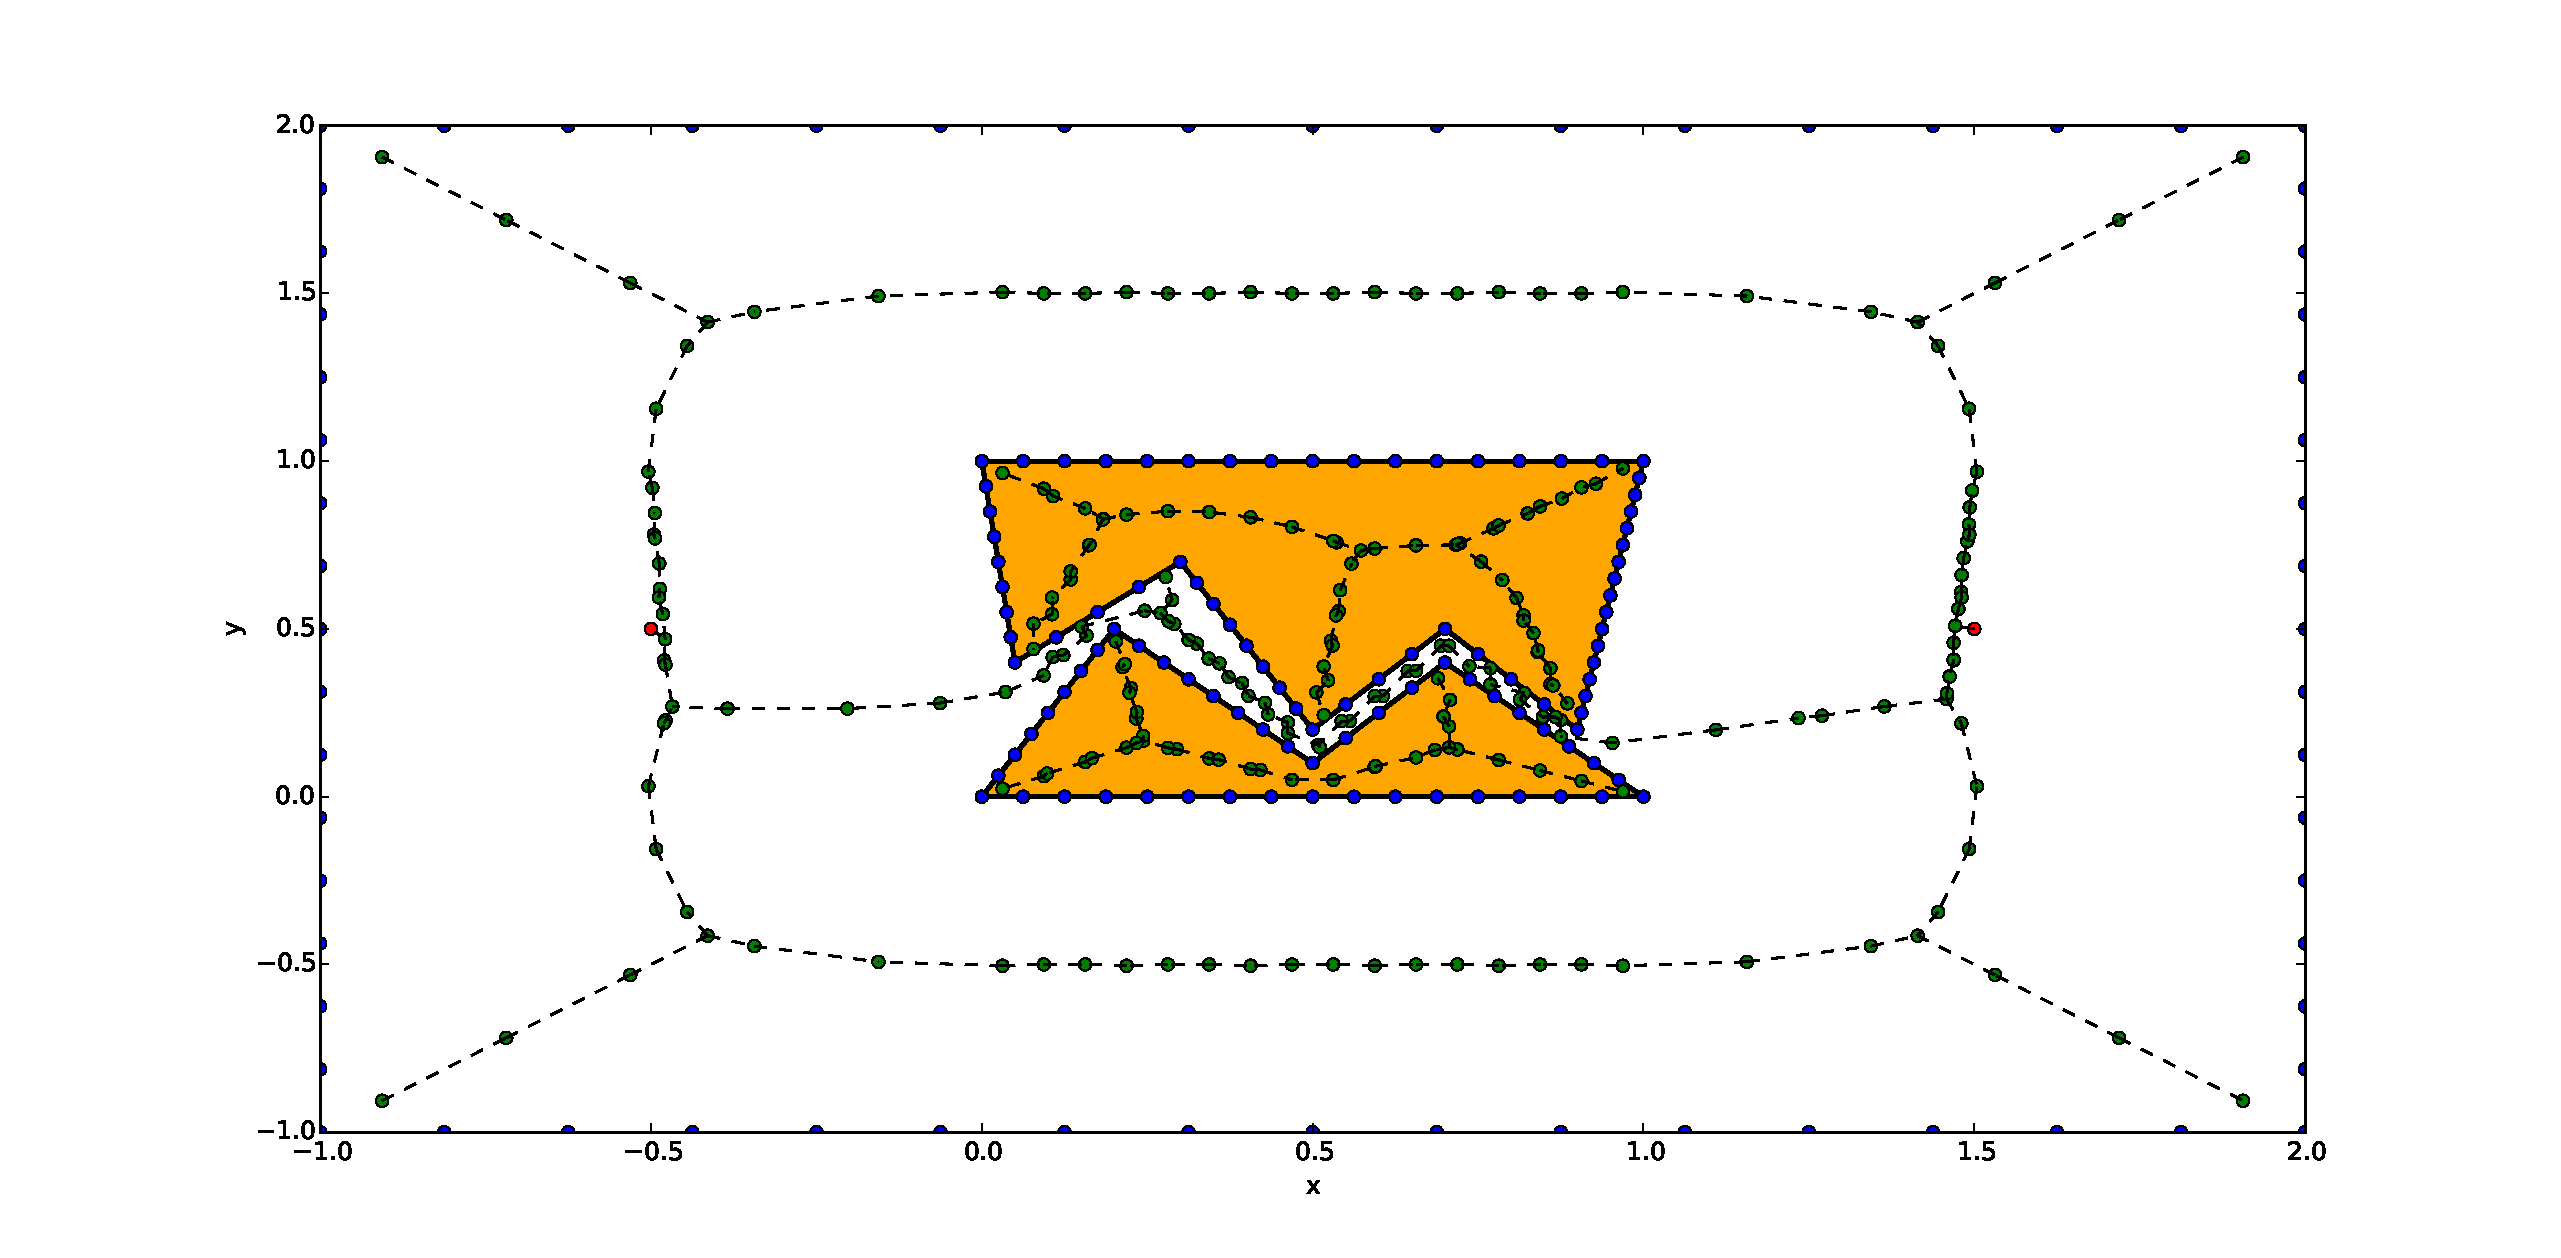
\includegraphics[width=\textwidth]{img/voronoi.pdf}
  \caption{Pruned Voronoi graph.}
  \label{fig:voronoi}
\end{figure}

In the figure the obstacles are the orange polygons; the bounding box
coincide with the border of the plot; the blue dots are the ones
distributed in point~\ref{item:distDots}; the green points are the
vertexes of the pruned voronoi diagram, constructed on
points~\ref{item:voronoi}, \ref{item:graph}, and~\ref{item:pruning};
the two red dots are the start and end vertexes added on point~\ref{item:startEnd}.
Note that there are also non influential disconnected graphs inside
the obstacles.

\subsubsection{Shortest path in graph}
The algorithm need to find a shortest path after the graph
generation. For doing that use the Dijkstra algorithm from the start
point to the end point.

\subsubsection{Normalization of path}
The purpose of the normalization phase is to have a path with vertexes
that have a certain distance between them.

In the specific the
algorithm go by all the vertexes of the shortest path, and measure the
distance from the previous vertex. If the distance is shorter than a
provided threshold merge the current and previous vertexes in
a single one located in the middle. If the distance is longer than
another provided threshold create a new vertex in the middle between
the current and the previous ones.

\subsection{Annealing}
The annealing phase is the key part of the algorithm, the purpose is
to make the initial path shorter, and on the same time keep the path
in a state where is possible to apply a specific spline without
colliding with obstacles.

\subsubsection{Spline}\label{sec:spline}

\subsubsection{Lagrangian relaxation in general}
A general constrained discrete optimization problem can be expressed in
the form:
\begin{equation}\label{eq:opt}
\begin{aligned}
& \underset{x}{\text{minimize}}
& & f(x) \\
& \text{subject to}
& & g(x)=0.
\end{aligned}
\end{equation}
Where $x$ is the state of the system in a discrete space $X$, $f(x)$
is the function to
minimize, and $g(x)=0$ is the constrain. the functions can also be
in a multidimensional discrete space, in that case the $x$ is a vector
$\mathbf{x}=(x_1,\dots,x_n)$ of variables.

For solving this class
of problem is necessary a \emph{Lagrange relaxation} method, that
augment the variable space $X$ by a \emph{Lagrange multiplier} space
$\Lambda$ of dimension equal to the number of constraints - one in the
problem~\eqref{eq:opt}.

The \emph{generalized discrete Lagrangian
  function} corresponding to the problem~\eqref{eq:opt} is:
\begin{equation}\label{eq:lagrangianFun}
  L_d(x,\lambda)=f(x)+\lambda H(h(x)).
\end{equation}
Where $\lambda$ is a variable in $\Lambda$, and if the dimension of
$\Lambda$ is more than one $\lambda$ must be transposed in
formula~\eqref{eq:lagrangianFun}; $H(x)$ is a non negative function
with the property that $H(0)=0$, the purpose is to transform $g(x)$ in
a non negative function - if $g(x)$ isn't already not negative - for
instance can be $H(g(x))=|g(x)|$ or $H(g(x))=h^2(x)$.

Under the previous assumptions the set of \emph{local minima}
in problem~\eqref{eq:opt} - that respect the constraints -  coincide
with the set of \emph{discrete saddle point}
in the augmented space. A point $(x^*,\lambda^*)$ is a discrete saddle
point if:
\begin{equation*}
  L_d(x^*,\lambda)\leq L_d(x^*,\lambda^*)\leq L_d(x,\lambda^*)
\end{equation*}
for all $x\in\mathcal{N}(x^*)$ and for all $\lambda\in\Lambda$, where
$\mathcal{N}(x^*)$ is the set of all neighbours of $x^*$.

\subsubsection{Lagrangian relaxation in project}
In the project the variable space $X$ is composed of all possible
configuration of the path, or in other words is the vector
$\mathbf{v}=(\mathbf{v}_1,\dots,\mathbf{v}_n)$ of all $n$ ordered
vertexes $\mathbf{v}_i=(x_i,y_i)$ of the
path. The problem~\eqref{eq:opt} is formulated in two different
versions in the project.
\begin{itemize}
\item The first one is:
  \begin{equation*}
    \begin{aligned}
      & \underset{\mathbf{v}}{\text{minimize}}
      & & length(\mathbf{v}) \\
      & \text{subject to}
      & & \left|bspline(\mathbf{v})\cap \bigcup_{i\in I}obstacle_i\right| = 0.
    \end{aligned}
  \end{equation*}
  Where $length(\mathbf{v})$ is the sum of the length of every edge of the
  path, that is the sum of the distances of every consecutive pair of
  vertexes $\mathbf{v_{i-1}}$ and $\mathbf{v_i}$; $bspline(\mathbf{v})$
  is the set of points of the \emph{B-Spline} obtained as explained in
  section~\ref{sec:spline} using the path as control polygon;
  $obstacle_i$ is the surface of the $i^{th}$ of $m$ obstacles, and
  $I=\{1,\dots,m\}$.
\item The second version is similar, but the function to minimize is
  $angle(\mathbf{v})$ instead of $length(\mathbf{v})$, where
  \begin{equation*}
    angle(\mathbf{v}) = \frac{\sum_{i=2}^{n-1}(1+\cos(\measuredangle \mathbf{v}_{i-1}\mathbf{v}_{i}\mathbf{v}_{i+1}))}{n-2},
  \end{equation*}
  and
  \begin{equation*}
    cos(\measuredangle
    \mathbf{v}_{i-1}\mathbf{v}_{i}\mathbf{v}_{i+1})=\frac{(\mathbf{v}_{i-1}-\mathbf{v}_{i})\cdot
      (\mathbf{v}_{i+1}-\mathbf{v}_{i})}{\|\mathbf{v}_{i-1}-\mathbf{v}_{i}\|\
      \|\mathbf{v}_{i+1}-\mathbf{v}_{i})\|}.
  \end{equation*}
\end{itemize}

The constraint function is not negative, and is calculated as the
ratio
\begin{equation*}
constraint(\mathbf{v}) = \frac{|\{\mathbf{p} \in spline(\mathbf{v})\ |\ \exists i\in\{1,\dots,m\}
  : \mathbf{p}\in obstacle_i \}|}{|\{\mathbf{p} \in spline(\mathbf{v})\}|}
\end{equation*}
where the points $\mathbf{p}$ of the spline are calculated in a discrete form. That
function is not negative, so the Lagrangian function correspondent to
equation~\eqref{eq:lagrangianFun} is
\begin{equation}\label{eq:lagrangianFunProj}
    L_d(\mathbf{v},\lambda)=length(\mathbf{v})+\lambda\cdot constraint(\mathbf{v}),
\end{equation}
or, alternatively, the correspondent one that use $angle(\mathbf{v})$ instead of $length(\mathbf{v})$.

\subsubsection{Annealing phase}
The target of the simulated annealing phase is to find the minimum
saddle points in
the curve represented by the
equation~\eqref{eq:lagrangianFunProj}.
\begin{algorithm}
 \caption{Annealing}\label{alg:annealing}
 \begin{algorithmic}[1]
   \Procedure{annealing}{$\mathbf{x}$}
   \State $\lambda\gets initialLambda$\label{alg:annealing:initialize}
   \State $T\gets initialTemperature$
   \While{not $terminationCondition()$}\label{alg:annealing:while}
   \For{number of trials}\label{alg:annealing:for}
   \State $changeLambda\gets$ true with $changeLambdaProb$\label{alg:annealing:lambdaProb}
   \If{$changeLambda$}
   \State $\lambda'\gets neighbour(\lambda)$\label{alg:annealing:changeLambda}
   \State $\lambda\gets \lambda'$ with probability $\me^{-([energy(\mathbf{x},\lambda)-energy(\mathbf{x},\lambda')]^+/T)}$
   \Else
   \State $\mathbf{x}'\gets neighbour(\mathbf{x})$\label{alg:annealing:changeX}
   \State $\mathbf{x}\gets \mathbf{x}'$ with probability $\me^{-([energy(\mathbf{x}',\lambda)-energy(\mathbf{x},\lambda)]^+/T)}$
   \EndIf
   \EndFor
   \State $T\gets T\cdot warmingRatio$\label{alg:annealing:cooling}
   \EndWhile
   \EndProcedure
 \end{algorithmic}
\end{algorithm}

The algorithm~\ref{alg:annealing} is the annealing process, on
line~\ref{alg:annealing:initialize} $\lambda$ and the
temperature are initialized; the \emph{while} on
line~\ref{alg:annealing:while} is the main loop and the terminating
condition\footnote{For the animation there isn't a terminating
  condition.} is given by a minimum temperature or a minimum variation of
energy between two iterations; the \emph{for} at
line~\ref{alg:annealing:for} repeat the annealing move for a certain
number of trials, on each iteration the algorithm probabilistically
try to make a move of the state of the system, first on
line~\ref{alg:annealing:lambdaProb} make a choice if moving in the
lagrangian space or in the space of the path, after that based on that
choice try to move the system in a neighbouring state - in the
lagrangian space at
line~\ref{alg:annealing:changeLambda} or in the path space at
line~\ref{alg:annealing:changeX} - the choice is made
probabilistically in the meaning that if the energy increase in the
lagrangian space or decrease in the path space the probability of
chosing the new state is 1, if the energy decrease in the lagrangian
space or increase in the path space then the new state is accepted
with a probability that is\footnote{Note that $[x]^+=\max(0,x)$.}:
$$\exp(-\frac{\Delta energy}{T}).$$
Finally at the end of every trial set,
at line~\ref{alg:annealing:cooling}, the temperature $T$ is cooled by
a certain factor.

The $neighbour$ function choose a neighbour of the state and is
defined depending on the input
\begin{itemize}
  \item for $\lambda$ move uniformly in a range $[-maxLambdaPert, maxLambdaPert]$;
  \item for path pick randomly one of the nodes, except the extremes,
    then pick an angle uniformly\footnote{Or with a
      gaussion with mean in the perpendicular direction of the two
      neighbouring points.} in $[0,2\pi]$.
\end{itemize}

The $energy$ function is equivalent of $L_d$ in the
equation~\eqref{eq:lagrangianFunProj}, the annealing process
find a saddle point probabilistically increasing the energy moving
$\lambda$ and 
decreasing the energy moving the points.

\begin{figure}[htb]
  \centering
  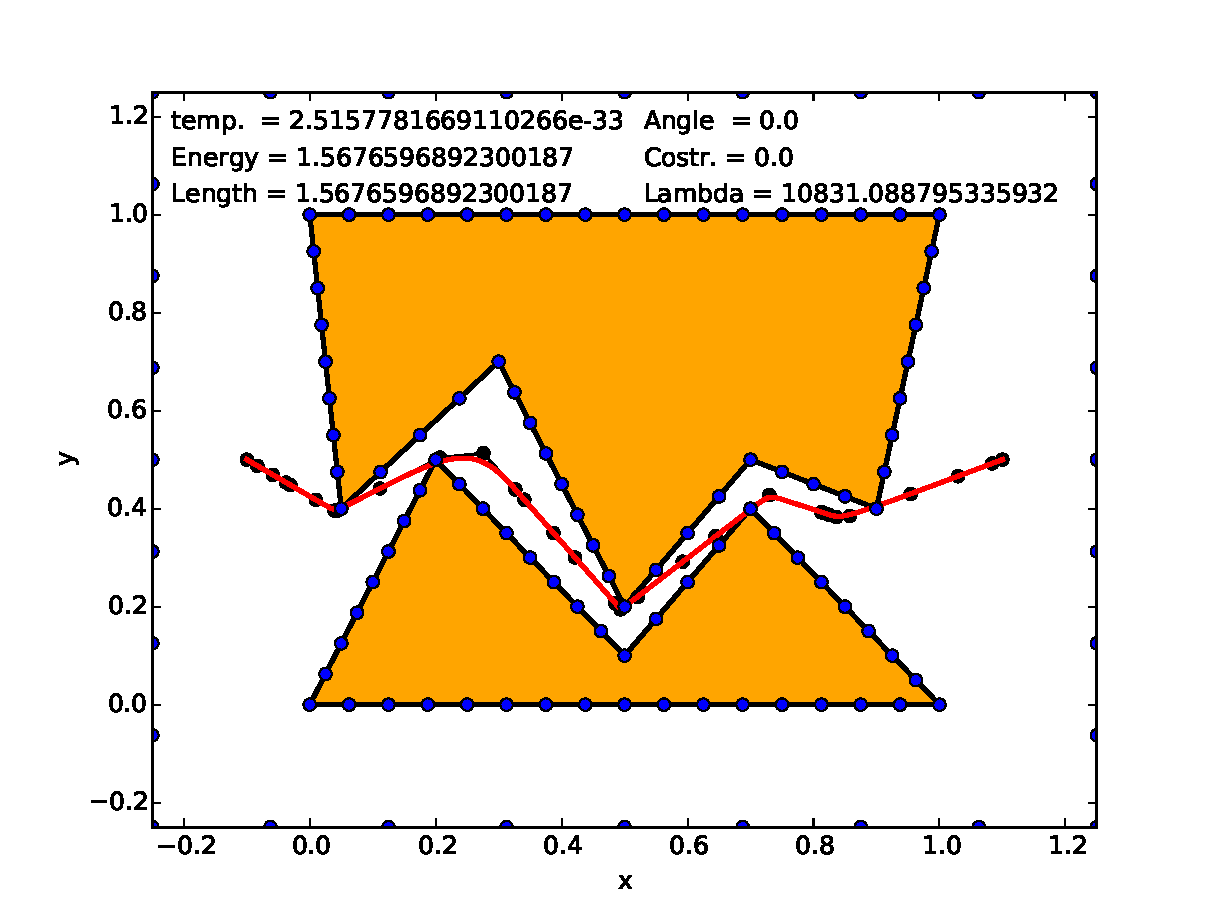
\includegraphics[width=\textwidth]{img/final.pdf}
  \caption{Final configuration after annealing.}
  \label{fig:final}
\end{figure}
In figure~\ref{fig:final} is visible the state of the system after a
certain amount of iterations.

\section{Conclusions}

\nocite{*}
\phantomsection
\addcontentsline{toc}{section}{\refname}
\bibliographystyle{apalike}
\bibliography{report}

\end{document}

